\documentclass[10pt,a4paper]{article}
\usepackage[utf8]{inputenc}
\usepackage{amsmath}
\usepackage{amsfonts}
\usepackage{amssymb}
\usepackage{geometry}
\usepackage{verbatim}
\usepackage{enumerate}
\usepackage{fancyvrb}
\usepackage{graphicx}
\usepackage{tikz}
\usepackage{hyperref}
\usetikzlibrary{positioning}
\usetikzlibrary{shapes,snakes}
\usepackage{nameref}

\usepackage[english]{babel}

\geometry{legalpaper, margin=1.5in}

\author{William Schultz}
\begin{document}
\title{Algorithms}
\author{William Schultz}
\maketitle

\newcommand{\concept}[1]{\textcolor{blue}{\textit{\textbf{#1}}}}

\section{Graph Search}

Can think about general graph search algorithm as consisting of an \textit{explored} set of nodes and a \textit{frontier} set of nodes. The goal is to eventually have the explored set equal to all nodes in the graph. The frontier is a set of nodes that we maintain along the way. Initially, we set the frontier to the starting node of the graph. It is unexplored but currently on our list of nodes that need to be explored i.e. it is on the frontier. We then pick a new node from the frontier set, mark it as explored, and do any other work we might need to do, and then take all of its neighbors and add them to the frontier set.

\subsection{Depth-first search}
Depth-first search searches deeper in a graph before searching broader. Can do a basic recursive or iterative implementation. Iterative implementation uses a stack to keep track of the frontier nodes, so that we explore deeper nodes first. We can also implement depth first search in a way that lets us recover paths to a node, by storing parent pointers as we go.

\subsection{Breadth-first search}
Breadth-first search searches all closer nodes before searching farther nodes i.e. it progresses in "levels" of depth. Not a standard way to implement it recursively, but can use a queue to keep track of the frontier nodes.

\section{Dynamic Programming}

There are 2 main components of a problem that make it amenable to a so-called ``dynamic programming'' (badly named) approach:
\begin{enumerate}
    \item \textbf{Optimal Substructure}: A global solution can be described in terms of solutions to smaller ``local'' problems. In other words, it is possible to find a solution to a larger problem by solving smaller problems and combine them in an efficient way. 
    \item \textbf{Overlapping Subproblems}: The global problem can be broken down into smaller ``local" sub-problems, and there is some overlap/redundancy between these subproblems, which is where you ideally get the efficiency speedup from.
\end{enumerate}
Note that either (1) and (2), in isolation, don't necessarily permit an efficient, dynamic programming based approach to a problem. For example, we can consider \textit{divide and conquer} type approaches as satisfying the \textit{optimal substructure} property, but don't necessarily satisfy the \textit{overlapping subproblems} property. For example, merge sort solves smaller subproblems (subsequences of an original list) and then merges them into a larger solution. But, in general, these smaller sorting problems cannot be expected to actually overlap at all.

Examples of problems with efficient DP approaches:
\begin{enumerate}
    \item \textbf{Fibonacci}: Compute the $n$-th Fibonacci number.
    \item \textbf{Subset Sum}: Given a set (multi-set) $S$ of integers and a target sum $k$, determine if there is a subset of $X \subseteq S$ such that the sum of integers in $X$ equals $k$.
    \item \textbf{Knapsack}: Given a set of $n$ items, each with a weight $w_i$ and values $v_i$, find a subset of items that fits in a knapsack of capacity $B$ and maximizes the overall value of included items.
    \item \textbf{Weighted Interval Scheduling}: Given a set of intervals $(s_i,e_i, W_i)$ represent as start and end times $s_i$ and $e_i$, respectively, and weight $W_i$, determine the maximum weight set of non-overlapping intervals.
    \item \textbf{Minimum Edit Distance}: Given two strings $S$ and $T$ over some alphabet of characters $\Sigma$, determine the minimum number of insertions or deletions needed to transform $S$ to $T$.
    \item \textbf{Matrix Chain Multiplication}: Given a sequence of matrices, determine the most efficient order in which to multiple them
\end{enumerate}


Can also look at some problems as having solution that can be built by a sequence of choices of which elements to add to the solution. This also allows for a more unified view in some cases between a greedy approach and a DP approach. For example, in the \textit{Subset Sum} problem, we can imagine a strategy where we build a solution by picking new elements from the original set to add to our output solution. We might take some kind of greedy approach where we, for example, pick the next smallest value and add it to our output. Clearly, the issue with the greedy approach in this problem is that it can get ``stuck'', with no next choices that allow the solution to be rectified, even if a solution does exist.

\subsection*{Stair Climbing}

This is an example of a somewhat simpler DP problem but is good to practice the basics. We are given a staircase, which can be represented as simply a sequence of $n$ steps, each with an associated cost. You can start at either the 0th or 1st step, and at each step you pay the cost of the current step and take either 1 or 2 steps up. Given these rules, you want to find the path up the stairs with minimal overall cost. This problem has a simple recursive breakdown that is simpler in character to other path finding problems, where the overall minimum cost solution can be represented in terms minimum cost solution to smaller paths of the original problem. Basically, if we say $\mathit{MinCost}(i)$ is the minimum cost solution starting from step index $i$, then we can represent this solution recursively as
\begin{align*}
    \mathit{MinCost}(i) = cost(i) + \mathit{Min}(\mathit{MinCost}(i+1), \mathit{MinCost}(i+2))
\end{align*}
while also accounting for the base case where $i > n$, in which case this means we've reached the top and can return cost 0.

If we expand the above recursion naively, though, it will contain an exponential number of calls, though there are many shared subproblems, similar to Fibonacci.
\begin{center}
    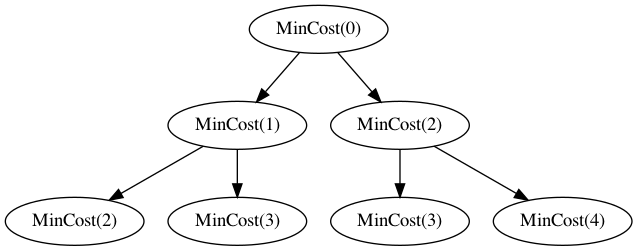
\includegraphics[scale=0.35]{diagrams/stairs_tree.png}
\end{center}
One simple approach here is to memoize solutions as we go, avoiding the exponential work blowup.


\subsection*{Subset Sum}
\label{sec:subset-sum}

To understand the idea behind approach for \textbf{Subset Sum}, can think about each element of the given list of $n$ integers $S=\{a_1,\dots,a_n\}$. If we wanted to come up with a naive recursive solution, we could imagine the decision tree for building all subsets of $S$, where each branch point represents whether we include that element or not in the subset. This is one way to simply generate all possible subsets of a given set. Within this tree, though, at each node, we can imagine we are dealing with a subset of the original set, based on the subset (e.g. suffix) of elements that we have not made a choice about including or excluding. Along with this, we can imagine that each node of the tree also has associated with it the ``used up'' amount, which is the sum of elements chosen to include based on the path to this position in the tree. Now, even though this tree naively has size (i.e, width) exponential in the number of elements, there are actually a limited number of unique problems to solve in this tree, so there is sufficient overlap between them to make this efficient.

Basically, if our target sum is $T$, then there are at most $T$ unique ``used up" values that can appear at any node in this tree. And, there are most $n$ unique suffixes that can appear as well.

% Note: not sure if I actually like the phrasing of the subproblem as ``suffixes''. Rather, we could imagine the subproblems as more generally being about 

\subsection*{Knapsack}

0-1 Knapsack is very similar to \nameref{sec:subset-sum} i.e., we have to find a subset of $n$ given items that remains under our given capacity and maximizes the sum of the chosen item values. Indeed, we can think of \textbf{Subset Sum} as a special case of the knapsack problem, where the values and weights of each element are the same. As in \textbf{Subset Sum} case, we can imagine a solution search tree where we either include or exclude the first element, and the subproblems we recurse on are basically the rest of the elements with a capacity reduced by that of our first element, or the rest of the elements with the original capacity. Again, this tree might grow exponentially, but, if our capacity is $C$, we actually only have at most $C$ unique possible capacities, and at most $n$ suffixes of elements. Note also that the minor difference from Subset Sum is that, when we combine solutions to recursive subproblems, we want to take the maximum solution (since this is an optimization problem variant), rather than just taking the disjunction.

\section*{Algorithms Problem List}

\subsubsection*{Product of Array Except Self}

\begin{itemize}
    \item \textbf{Problem}: Given an array of integers, $S$, compute an output array $A$ such that $A[i]$ is equal to the product of all integers in $S$ excluding $S[i]$.
    \item \textbf{Solution Idea}: The naive solution is to go over every index $i$ in $S$ and compute the product of all other indices in $S$ and set $A[i]$ equal to this product. The downside is that this is not so efficient, since it takes $O(n^2)$ time in the worst case, if $n$ is the length of the input array $S$. The key goal is to see if we can somehow do this more efficiently. 
    
    One way to think about this is to consider the multiplications we are doing in the brute force solution e.g. if we have an array $S=\{1,2,3,4\}$ and we consider the multiplications being done at each index:
    \begin{align*}
        i=0 : \, \, (\phantom{1 \cdot} 2 \cdot 3 \cdot 4) \\ 
        i=1 : \, \, (1 \phantom{1 \cdot} \cdot 3 \cdot 4) \\
        i=2 : \, \, (1 \cdot 2 \phantom{1 \cdot} \cdot 4) \\
        i=3 : \, \, (1 \cdot 2 \cdot 3 \phantom{1 \cdot})
    \end{align*}
    It seems like we are doing some repeated work across this set of different multiplications. For example, the multiplication pair $2 \cdot 3$ occurs at index $0$ and index $3$, and the pair $1 \cdot 3$ occurs at indices $1$ and $3$. This would seem to imply that we only need to do these sub-multiplications once, and can then cache the results each time we need them. 
    
    More generally, we can actually observe that each index in the output array can be represented more succintly as a product of a \textit{prefix} and \textit{suffix} of the input array. And, each of these prefixes and suffixes are, then, naturally nested subproblems relative to each other, so if we compute the product of one prefix, we can compute the product of the next larger prefix without re-computing the whole prefix product from scratch. So, the essential idea is that if we can go through, in linear time, and compute these prefix and suffix products for each index of the input array, then we can go again and compute the values for each index of the output array with one scan, by simply multiplying the appropriate prefix and suffix product together.

    % Table representing matrix with numbers 1,2,3,4,5 in rows and columns.
    \begin{center}
        \begin{tabular}{c|c|c|c|c|c}
             &  &  &  &  &  (prefix) $\cdot$ (suffix) \\
             \hline
            - & 2 & 3 & 4 & 5 & = $(2 \cdot 3 \cdot 4 \cdot 5)$\\
            \hline
            1 & - & 3 & 4 & 5 & = $(1) \cdot (3 \cdot 4 \cdot 5)$ \\
            \hline
            1 & 2 & - & 4 & 5 & = $(1 \cdot 2) \cdot  (4 \cdot 5)$ \\
            \hline
            1 & 2 & 3 & - & 5 & = $(1 \cdot 2 \cdot 3) \cdot (5)$ \\
            \hline
            1 & 2 & 3 & 4 & - & = $(1 \cdot 2 \cdot 3 \cdot 4)$ \\
        \end{tabular}
    \end{center}
\end{itemize}



\subsubsection*{Increasing Triplet Subsequence}

\begin{itemize}
    \item \textbf{Problem}: Given an integer array $nums$, return \textit{true} if there exists a triple of indices $i,j,k$ such that $i < j < k$ and $nums[i] < nums[j] < nums[k]$.
    \item \textbf{Solution Idea}: A brute force way to compute this would be to loop over all indices $i$, and, for each, first search for $j > i$ such that $nums[j] > nums[i]$. If found, then start from $j$ and search for $k > j$ such that $nums[k] > nums[j]$. Actually, what is the worst case running time of this solution? In the worst, case, I think this would be $O(n^3)$, since for each index, we may need to search $n$ other indices, and we are doing this both for $j$ w.r.t $i$ and $k$ w.r.t $j$, in the worst case.
    
    Ok, note a key insight: for \textit{any} valid increasing triplet subsequence, there must also be such a valid triplet that includes the smallest (and second smallest) element of the array. So, we can utilize this insight to maintain only a conservative lower bound for the possible triplet subsequences i.e., we really only need to maintain the two smallest elements in order to check for possible triplet subsequences. Essentially, checking for a triplet subsequence with some $i,j,k$ for which there exists an $i' < i$ s.t. $nums[i'] < nums[i]$ is actually wasteful, if we've already checked it for $(i',j,k)$.
\end{itemize}


\subsubsection*{Difference of Two Arrays}
\begin{itemize}
    \item \textbf{Problem}: Given two integer arrays $S_1$ and $S_2$, return sets $U_1,U_2$ where $U_1$ is the set of distinct integers in $S_1$ and not in $S_2$, and $U_2$ is the set of distinct integers in $S_2$ and not in $S_1$.
\end{itemize}

\subsubsection*{Merge Strings Alternately}
\begin{itemize}
    \item \textbf{Problem}: Given two strings $s_1$ and $s_2$, merge them into one string $S$ such that the output string $S$ interleaves the characters of $s_1$ and $s_2$ alternately. If one string is longer than the other, then we append the remaining characters of that string to the end of the output string.
\end{itemize}


\subsubsection*{Greatest Common Divisor of Strings}
\begin{itemize}
    \item \textbf{Problem}: Given two strings $s$ and $t$, we say that $t$ ``divides'' $s$ if $s = t + t + \dots + t$. That is, $s$ consists of $t$ concateneated with  itself 1 or more times. Given two strings $s_1$ and $s_2$, we want to find the greatest common divisor $x$ between $s_1$ and $s_2$. That is, the largest string $x$ such that $x$ divides $s_1$ and $s_2$.
\end{itemize}

\subsubsection*{Kids with Greatest Number of Candies}
\begin{itemize}
    \item \textbf{Problem}: Given array of kids with some number of candies, and number of extra candides, compute whehter each kid would have max candies after receiving the number of extra candies you have.
\end{itemize}

\subsubsection*{Merge k Sorted Lists}

\begin{itemize}
    \item \textbf{Problem}: Given a set of $k$ linked lists, each which are individually sorted in ascending order, merge all $k$ lists into one sorted list. 
    \item \textbf{Solution Idea}: The basic approach is to essentially just perform the \textit{merge} step of merge-sort. That is, if we are given a set of already sorted lists, we can merge them all into one sorted lists by repeatedly popping the smallest element from the remaining, non-empty lists and appending it to the output list.
    \item \textbf{Key Concepts}: 
    \begin{itemize}
        \item \concept{Mergesort Merging}
        \item \concept{Linked List Manipulation}
    \end{itemize}
    The essence of the solution is very straightforward as long as you know and understand the ideas behind mergesort i.e. knowing the core idea that you can merge a set of already sorted lists by incrementally choosing the smallest element from each.
\end{itemize}

\subsubsection*{Remove duplicates from sorted linked list}
\begin{itemize}
\item \textbf{Problem}: Given a sorted linked list, remove any duplicates from the list.
\item \textbf{Solution Idea}: Iterate through the linked list, but at each node look ahead to see how many nodes in front of you contain an identical value to your own. Update your current ``next" pointer to point to the first node after this block of identical nodes in front of you. Since the list is sorted, you know that any duplicates of the current value must be directly in front of you.
\item \textbf{Key Concepts}: 
\begin{itemize}
    \item \concept{Linked List Traversal}
    \item \concept{Linked List Deletion}
    \item \concept{Duplicate Detection by Sorting}
\end{itemize}
The underlying insight in the solution is to recognize that sorting a list can be used an easy mechanism for detecting duplicates. That is, in a sorted list, all duplicates of a particular item will always appear in contiguous ``blocks". Once you recognize this fact, then implementing the solution mostly requires a standard application of linked list iteration and linked list item deletion. Namely, that to delete an item $n_2$ from a linked list that appears in a list as $n1 \rightarrow n_2 \rightarrow n_3$, you simply update  the ``next" pointer of $n_1$ to point to $n_3$ instead of $n_2$. Recall that a basic linked list node is a $LinkedListNode(val, next)$ structure, where $val$ is the value of that node, and $next$ is a pointer to the next item in the list.
\end{itemize}

\subsubsection*{Intersection of two linked lists}
\begin{itemize}
\item \textbf{Problem}: Given two singly linked lists, return the node at which the two lists intersect. If they have no intersection, then return \textit{null}.
\item \textbf{Solution Idea}: This is similar to a \textit{lowest common ancestor} problem. One approach is to walk backwards to the root from one of the lists and keep track of all nodes seen along the way. Then, walk backwards from the other list and check for the first node you hit that was already seen, and that node should be the intersection point. Note that this uses $O(n)$ space, if $n$ the upper bound on the size of the linked lists. 

It's also possible to do it without using any extra space by using a cleverer 2 pointer approach with a bit of counting. If we walk back to the root in both lists we can record the longer of the two. Then, from this we know the difference in length between the two lists, $diff$. So, we can walk backwards by $diff$ pointers in the longer list, and then walk forwards from there in both lists at the same time, until we hit a point where both pointers are pointing to the same node.
\item \textbf{Key Concepts}:
\begin{itemize}
    \item \concept{Linked List Traversal}
    \item \concept{Lowest Common Ancestor (?)}
\end{itemize}
\end{itemize}

\subsubsection*{Reverse linked list}
\begin{itemize}
\item \textbf{Problem}: Given a singly linked list, reverse the list.
\item \textbf{Solution Idea}: Iterate over the list and at each node, re-arrange the \textit{next} pointer so it now points to the previous node rather than the next node.
\begin{align*}
    None \rightarrow a \rightarrow b \rightarrow c
\end{align*}
If $curr=a$ and $curr.next = b$, then to do the reversal we want to end up with $a.next = None$ and then step forward, ending up with $curr=b$. So, at each step of the traversal, we keep track of hte previous item we looked at, so that we can reverse the pointer of the current node to point to it. We also need to save a reference to the next node before we update it.
\item \textbf{Key Concepts}:
\begin{itemize}
    \item \concept{Linked List Traversal}
    \item \concept{Pointer Swapping (?)}
\end{itemize}
Need to have a solid grasp of how to traverse a linked list, but also need to have good confidence in how to update points in a few steps (similar to how we swap variables), without overwriting the info we need to continue.
\end{itemize}

\subsubsection*{Add two binary strings}
% \begin{itemize}
% \item \textbf{Problem}: Given a singly linked list, reverse the list.
% \item \textbf{Solution Idea}: Iterate over the list and at each node, re-arrange the \textit{next} pointer so it now points to the previous node rather than the next node.
% \begin{align*}
%     None \rightarrow a \rightarrow b \rightarrow c
% \end{align*}
% If $curr=a$ and $curr.next = b$, then to do the reversal we want to end up with $a.next = None$ and then step forward, ending up with $curr=b$. So, at each step of the traversal, we keep track of hte previous item we looked at, so that we can reverse the pointer of the current node to point to it. We also need to save a reference to the next node before we update it.
% \item \textbf{Key Concepts}:
% \begin{itemize}
%     \item \concept{Linked List Traversal}
%     \item \concept{Pointer Swapping (?)}
% \end{itemize}
% Need to have a solid grasp of how to traverse a linked list, but also need to have good confidence in how to update points in a few steps (similar to how we swap variables), without overwriting the info we need to continue.
% \end{itemize}

\subsubsection*{Subsets of a list}

% \bibliographystyle{plain}
% \bibliography{../../references.bib}

\end{document}